\documentclass[9pt]{beamer}
\usepackage[boldfont]{xeCJK}
\usepackage{mathtools}
\usepackage{amsmath, amssymb, amsthm}
\usepackage{mathpartir}
\usepackage{lstautogobble}
\usepackage{syntax}
\usepackage{listings}
\usepackage{xcolor}
\usepackage{indentfirst}
\usepackage{tikz}
\usepackage{shorttoc}

\usetheme{Copenhagen}
\newcommand{\xto}{\xrightarrow}
\let\emptyset\varnothing

\setmainfont[Scale=1.08]{Charter}
\setCJKmainfont[Scale=1.15]{STSong}
\setCJKfamilyfont{kai}{Kaiti SC}

\newfontfamily\listingsfont{PT Mono}

\linespread{1.3}
\lstset{
        basicstyle=\listingsfont\linespread{0.1},
        keywordstyle=\bfseries\color{blue},
        commentstyle=\itshape\color{gray},
        numberstyle=\color{black}
}
\lstdefinelanguage{Ocaml}{morekeywords={fun, let, in,if,then,else}}

\title{基于Hindley-Milner类型系统的控制流分析算法}
\author[Xiangyu Luo]{罗翔宇}
\institute[sist]{北京大学\\信息科学技术学院}

\begin{document}
    \begin{frame}
        \titlepage
    \end{frame}
    
    \section{背景介绍}
    \begin{frame}{控制流分析}
        \begin{itemize}
        		\item 当今程序的静态分析在软件工程领域扮演了越来越重要的角色,代码漏洞检测、代码优化等都离不开程序静态分析的结果
		\vspace{0.8em}
		\item 而控制流分析是静态分析一个最基础的环节,有了控制流分析的结果,就可以做数据流分析、程序切片等静态分析
        \end{itemize}
    \end{frame}
    
\begin{frame}[fragile]{函数式语言的控制流分析}
    	\begin{itemize}
		\item 命令式语言的控制流分析结果一般都是划分基本块并画出控制流图
				\vspace{0.8em}
		\item 函数式语言中,由于没有类似于命令式语言自顶向下的求值顺序,故函数式语言上的控制流分析一般指确定函数的调用目标。
        \begin{lstlisting}[language=Ocaml]
	let f = fun x -> if x then False else True
	in f True
        \end{lstlisting}
        \end{itemize}
        更一般的定义为:在函数式语言中,一个表达式的控制流分析结果即为该表达式最终求值的可能结果的集合。
\end{frame}
    
\begin{frame}{基于类型系统的控制流分析}
	\begin{itemize}
		\item 基于类型系统的控制流分析相比于基于抽象解释的控制流分析,有着效率高、模块化强、求值顺序无关等特点。
		\vspace{0.8em}
		\item Hindley-Milner是在函数式语言里广泛应用的类型系统,但是目前并没有在其上运行的控制流分析算法。
	\end{itemize}
\end{frame}

\begin{frame}{Hindley-Milner 类型系统}
	目前Haskell, Ocaml等主流函数式编程语言的类型系统都基于Hindley-Milner类型系统。相比于其它类型系统,它有以下两个特点:
	\vspace{1.5em}
	\begin{itemize}
		\item 函数参数类型免于声明,可以通过类型重建重建出
		\item let语句绑定的变量都具有多态性
	\end{itemize}
	\vspace{1.5em}
	这两个特点为开发人员编写程序提供了极大的便利,但是也为我们的控制流分析带来了巨大的挑战。
\end{frame}

\begin{frame}[fragile]{算法框架}
	\begin{itemize}
		\item 我们的算法基于扩展的带有流属性的类型系统。
		\vspace{0.5em}
		\item 所谓流属性类型即为每一个原始类型都绑定一个标号集合,表明拥有该类型的表达式,最终可能的求值结果的标号集合。
		\item 带标号的程序示例:
		\begin{lstlisting}[language=Ocaml, escapeinside={`}{`}]
(fun`$^{\ell_1}$` x -> if`$^{\ell_2}$` x`$^{\ell_3}$` then True`$^{\ell_4}$` else False`$^{\ell_5}$`) True`$^{\ell_6}$`
		\end{lstlisting}
		\item 这里使用我们的算法可以推导出前面函数的类型为$Bool^{\ \ell_6}\xrightarrow{\ell_1}Bool^{\ \{\ell_4, \ell_5\}}$, 整个表达式的类型为$Bool^{\ \{\ell_4, \ell_5\}}$
	\end{itemize}
	\vspace{0.2em}
	由于所有子表达式的标号都是互不相同的,故一旦完成了类型推导,就可以根据表达类型得到其控制流分析的结果。
\end{frame}

\begin{frame}[fragile]{HM类型系统的参数类型重建}
	\begin{itemize}
		\item HM类型系统中,所有的函数参数均可以不用声明类型。
		\vspace{0.3em}
		\item 我们要为每一个函数参数分配一个类型变量,然后在根据参数的使用将对应的参数变量添加进一个类型约束集合,最终解类型约束集合得到每个类型变量所代表的真实类型。
		\vspace{0.3em}
		\item 除了类型变量,我们需要一个流属性变量来代指任何类型的流属性。维护类型约束集合的同时也要维护一个流属性约束集合,最终求解流属性约束集合。
		\vspace{0.3em}
		\item 代码示例: 
	\end{itemize}
\end{frame}

\begin{frame}[fragile]{HM类型系统中的参数类型重建}
	\begin{itemize}
		\item 考虑函数:
		\begin{lstlisting}[language=Ocaml, escapeinside={`}{`}]
		fun x -> x True`$^{\ell_1}$`
		\end{lstlisting}
		\item 这里这里我们为变量x分配一个类型变量$X$,流属性变量$\alpha$,故x有类型$X^{\ \alpha}$,类型约束集合为$\{X = Bool \to Y\}$, 流属性约束集合为$\{\{\ell_1\}\subseteq\alpha\}$
		\vspace{0.3em}
		\item 事实上这根据流属性的包含关系构成了一个子类型系统,我们只需要维护子类型的关系,然后根据子类型关系再次推导出流属性之间的包含关系即可。
	\end{itemize}
\end{frame}

\begin{frame}[fragile]{类型变量实例化}
	\begin{itemize}
		\item 一个问题是,我们不能简单地将类型变量直接实例化为类型
		\begin{lstlisting}[language=Ocaml,escapeinside={`}{`}]
			if True then fun`$^{\ \ell_1}$` x -> True`$^{\ \ell_3}$` else fun`$^{\ \ell_2}$` x -> False`$^{\ \ell_4}$`
		\end{lstlisting}
		\vspace{0.2em}
		\item 考虑如上代码,我们有类型约束集合$\{X^{\ \alpha} = Y^{\ \beta}\xrightarrow{\{\ell_1\}}Bool^{\{\ell_3\}}\}$和$\{X^{\ \alpha} = Z^{\ \gamma}\xrightarrow{\{\ell_2\}}Bool^{\{\ell_4\}}\}$。 子类型约束集合:$\{X^{\ \alpha} \succeq Y^{\ \beta}\xrightarrow{\{\ell_1\}}Bool^{\{\ell_3\}}\}$和$\{X^{\ \alpha} \succeq Z^{\ \gamma}\xrightarrow{\{\ell_2\}}Bool^{\{\ell_4\}}\}$
		\vspace{0.2em}
		\item 如果我们简单地把$X$替换,就会在子类型约束集合中导出矛盾。所以我们需要在替换时只替换类型,而把所有的流属性用新的流属性变量替代。
	\end{itemize}
\end{frame}

\begin{frame}[fragile]{let多态绑定}
	\begin{itemize}
		\item 在Hindley-Milner类型系统中,处理let多态的方式为,先求出绑定的表达式的主类型T,以及记录当前表达式产生的类型约束集合S。
		\vspace{0.2em}
		\item 求解约束集合S,并将其解应用到当前环境和后续的分析过程中。
		\vspace{0.2em}
		\item 但是由于子类型约束集合不能部分求解, 所以我们需要将集合记录在类型中。
	\end{itemize}
\end{frame}

\begin{frame}[fragile]{流属性类型模板}
	\begin{itemize}
		\item 我们创造形如$\forall \vec{\alpha}.C\Rightarrow T$, 表示对于所有满足子类型约束集合的流属性$\vec{\ell}$,有类型$T[\vec{\alpha}/\vec{\ell}]$
		\vspace{0.2em}
		\item 对于let语句,我们首先分析绑定的表达式,得到其类型$T$,和子类型约束集合$C$,然后令绑定的变量类型为形如的$\forall\vec{\alpha}.C\Rightarrow T$, 其中$\vec{\alpha}$为$T$中所有自由出现的流属性变量。
		\vspace{0.2em}
		\item 实例化流属性类型模板是,首先新建流属性变量$\vec{\beta}$,然后得到类型$T[\vec{\alpha}/\vec{\beta}]$,和流属性约束集合$C[\vec{\alpha}/\vec{\beta}]$
	\end{itemize}
\end{frame}

\begin{frame}[fragile]{约束集合指数爆炸}
	\begin{itemize}
		\item 考虑如下程序
		\begin{lstlisting}[escapeinside={`}{`}, language=Ocaml]
	let x0 = e in
		let x1 = fun y -> if y then x0 else x0 in
			let x2 = fun z -> if z then x1 else x1 in
				...
		\end{lstlisting}
		\item 不妨设推导e时,产生了流属性约束集合$C_0$,接下来推导x1的绑定表达式时,其约束集合$C_1$中包含$C_0$的两个拷贝,而同理$C_2$中也包含$C_1$的两个拷贝
		\vspace{0.3em}
		\item 流属性约束集合的大小随着let的嵌套层数而指数爆炸
	\end{itemize}
\end{frame}

\begin{frame}[fragile]{合并冗余约束}
	可以发现有一些约束是多余的,可以将其合并为一条约束:
	\vspace{0.5em}
	\begin{itemize}
				\item 如果约束集合中存在$\{\ell_1\subseteq \alpha, \ell_2\subseteq \alpha\}$的约束,可以将其合并为$\{\ell_1\cup\ell_2 \subseteq \alpha\}$. 
		\vspace{0.3em}
		\item 如果约束集合中存在$\{\ell_1 \subseteq \alpha, \ell_2 \subseteq \alpha, \alpha\subseteq \beta\}$,且$\alpha$在表达式无自由出现,那么可以将其合并为$\{\ell_1\cup\ell_2\subseteq\beta\}$
	\end{itemize}
	\vspace{0.5em}
	可以发现合并过约束之后,流属性约束集合中变量的个数最多只有$O(n)$个,故最多有$O(n^2)$条约束
\end{frame}

\begin{frame}[fragile]{求解流属性约束}
	\begin{itemize}
		\item 我们可以将流属性约束转化为一个图来进行求解。
		\vspace{0.3em}
		\item 如果有约束$\{\alpha\preceq\beta\}$, 则在其之间连接一条有向边
		\vspace{0.3em}
		\item 可以发现一个变量所代表的流属性集合,即是它在此图中可以到达的所有顶点的流属性集合的并集
	\end{itemize}
\end{frame}

\begin{frame}[fragile]{求解流属性约束}
	\begin{itemize}
		\item 我们先考虑这个图没有环的情况,此时该图可以拓扑排序,然后按照拓扑排序的结果使用动态规划求解即可。
		\vspace{0.5em}
		\begin{center}
	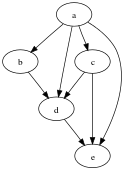
\includegraphics[width=1.8cm]{DAG.png}
	\end{center}
		\vspace{0.2em}
		\item 如果有环的话,我们可以使用Tarjan算法收缩图的极大强连通分量,然后在收缩过的新图上使用有向无环图的算法求解,再根据原图顶点和强连通分量之间的对应关系,计算出原图顶点的流属性集合。
	\end{itemize}
\end{frame}
	
\begin{frame}[fragile]{形式化类型推导规则}
	\begin{mathparpagebreakable}
			\inferrule{x:\tau\in A\quad\mathrm{let}\ \varphi\ \mathrm{be}\ instantiate_f(\tau)\ \mathrm{and}\ C\ \mathrm{be}\ generalize_c(\tau)}{A\vdash x:instantiate_t(\varphi)\mid \emptyset\mid C} \qquad\mathrm{Id}\and
		\inferrule{X\ \mathrm{is\ a\ fresh\ type\ variable}\quad A, x:X\vdash e:\kappa\mid D\mid C}{A\vdash \lambda^{l}x.e:X\xto{\{l\}} \kappa\mid D \mid C}\qquad\mathrm{Abs}\and
		\inferrule{A\vdash e_1:\kappa_1\mid D_1\mid C_1\quad A\vdash e_2:\kappa_2\mid D_1\mid C_1\\ \mathrm{X\ is\ a\ fresh\ type\ variable}\quad\mathrm{\alpha\ is\ a\ fresh\ flow\ properties\ variable}}{A\vdash e_1\ e_2:X\mid D_1\cup D_2\cup \{\kappa_1 = \kappa_2\xto{\alpha} X\}\mid C_1\cup C_2\cup \{\kappa1 \preceq \kappa_2\xto{\alpha}X\}}\qquad\mathrm{App}\and
	\end{mathparpagebreakable}
\end{frame}

\begin{frame}[fragile]{形式化类型推导规则}
\begin{mathparpagebreakable}
			\inferrule{\mathrm{X\ is\ a\ fresh\ type\ variable}\quad A,x:\kappa\vdash e:\kappa\mid D\mid C}{A\vdash \mathrm{fix}\,x.e:\kappa\mid C\cup\{\kappa=X\}\mid D\cup\{\kappa\preceq X\}}\qquad\mathrm{Fix}\and
		\inferrule{A\vdash e_1:\kappa_1\mid D_1\mid C_1\quad A\vdash e_2:\kappa_2\mid D_2\mid C_2}{A\vdash (e_1,e_2)^{l}:(\kappa_1, \kappa_2)^{\{l\}}\mid D_1\cup D_2\mid C_1\cup C_2}\qquad\mathrm{Tuple}\and
		\inferrule{A\vdash e:(\kappa_1, \kappa_2)^{\alpha}\mid D_1\mid C_1\quad A,x:\kappa_1,y:\kappa_2\vdash e':\kappa_3\mid D_2\mid C_2}{A\vdash\mathrm{let}\ (x,y)=e\ \mathrm{in}\ e':\kappa_3\mid C_1\cup C_2\mid D_1\cup D_2}\qquad\mathrm{Tuple\ Decons}\and
		\inferrule{A\vdash e:\kappa\mid D\mid C\quad \mathrm{let}\ S\ \mathrm{be\ the\ solution\ of}\ D\quad \\ S(A), x:S(generalize_f(S(A), C, generalize_t(S(A), \kappa)))\vdash e':\kappa'\mid D'\mid C'}{A\vdash\mathrm{let}\ x=e\ \mathrm{in}\ e':\kappa' \mid D\cup D'\mid C\cup C'}\qquad\mathrm{Let}\and
\end{mathparpagebreakable}
\end{frame}

\begin{frame}[fragile]{形式化类型推导规则}
	\begin{mathparpagebreakable}
			\inferrule{\mathrm{\alpha\ is\ a\ fresh\ flow\ properties\ variable}\quad X\ \mathrm{is\ a\ fresh\ type\ variable}\\ A\vdash e_1:\kappa_1\mid D_1\mid C_1\quad A\vdash e_2:\kappa_2\mid D_2\mid C_2\quad A\vdash e_3:\kappa_3\mid D_3\mid C_3}{A\vdash \mathrm{if}\ e_1\ \mathrm{then}\ e_2\ \mathrm{else}\ e_3:X \mid D_1\cup\\ D_2\cup D_3\cup \{\kappa_1=Bool^\alpha, \kappa_2=\kappa_3\}\mid C_1\cup C_2\cup C_3\cup \{\kappa_2\preceq X, \kappa_3\preceq X\}}\qquad\mathrm{If}\and
		\inferrule{}{A\vdash True^l:Bool^{\{l\}}\mid\emptyset\mid\emptyset}\qquad\mathrm{True}\and
		\inferrule{}{A\vdash False^l:Bool^{\{l\}}\mid\emptyset\mid\emptyset}\qquad\mathrm{False}\and
		\inferrule{x\in\{1,2,\cdots\}}{A\vdash x^l:Int^{\{l\}}\mid\emptyset\mid\emptyset}\qquad\mathrm{Int}

	\end{mathparpagebreakable}
\end{frame}

\begin{frame}[fragile]{试验评测}
	\begin{itemize}
		\item 在实验中,我们为了用户方便起见,定义一个表达式的标号为这个表达式在源代码中的位置。
		\vspace{0.3em}
		\item 	我们一共有小、中、大四个测试文件,其中小测试样例只用于在论文中说明我们测试的方法,代码如下:
		
	\begin{lstlisting}
	        let f = \x -> if x then 1 else 2 in
	        f True
	\end{lstlisting}
		\item 我们有输出:
	\end{itemize}
\end{frame}

\begin{frame}[fragile]{试验输出}
	\begin{itemize}
			\item\begin{lstlisting}
[(1,18),(1,20)] -> [(2,3),(3,1)],
[(1,25),(1,27)] -> [(1,25),(1,27)],
[(1,32),(1,34)] -> [(1,32),(1,34)],
[(1,15),(1,34)] -> [(1,25),(1,27)], [(1,32),(1,34)],
[(1,9),(1,34)] -> [(1,9),(1,34)],
[(2,1),(2,3)] -> [(1,9),(1,34)],
[(2,3),(3,1)] -> [(2,3),(3,1)],
[(2,1),(3,1)] -> [(1,25),(1,27)], [(1,32),(1,34)],
[(1,1),(3,1)] -> [(1,25),(1,27)], [(1,32),(1,34)],
	\end{lstlisting}

	\end{itemize}
\end{frame}

\begin{frame}[fragile]{试验评测}
	\begin{itemize}
		\item 其中medium.hs文件由20层嵌套的let语句组成,为了测试let嵌套时的运行效率,防止约束集合指数爆炸。
		\vspace{0.2em}
		\item 这个测试文件在0.098秒内即可运行出解,说明我们针对let嵌套的优化有效。
		\vspace{0.5em}
		\item 而large.hs文件由107行haskell代码构成,其中包含ski组合子、基于$\lambda$演算定义的邱奇数、基于$\lambda$演算定义的元组函数、列表函数等各种较为复杂的函数。
		\vspace{0.2em}
		\item 经过分析,我们的控制流算法共分析出了1319处目标函数调用的结果,而CPA则分析出有1996处目标函数调用结果,相当于将CPA的准确度提升了$34\%$。
		\vspace{0.2em}
		\item 注意到CPA随着程序代码量的上升,准确度会进一步下降,故我们的算法在分析更大规模的程序时,相比于CPA的准确度会进一步提高。
	\end{itemize}
\end{frame}

\begin{frame}[fragile]{提问环节}
	\begin{itemize}
		\item Thank you 
		\vspace{1em}
		\item Q\&A
	\end{itemize}
\end{frame}

\end{document}
